\chapter{Basics of Sweet.JS}
\textcolor{white}{``}Sweet.JS~\cite{bib6} is a hygienic macro compiler for JavaScript that takes JavaScript macros and produces normal JavaScript code that one can run in a browser or using a standalone interpreter like Node.JS. The idea is that you define a macro with a name and a list of patterns. Whenever a macro is invoked, the code is matched and expanded at  compile time and produces the expanded source that can be run in any JavaScript environment. \textcolor{white}{''}
\section{Types of macros in Sweet.JS}
\begin{enumerate}
\item {\bf Rule macros }
Rule macros work by matching a syntax pattern and generating new syntax based on the template.
To define a rule base macro the grammar is
\begin{lstlisting}[frame=single]
macro <name> {
  rule { <pattern> } => { <template> }
}
\end{lstlisting} 

The following macro defines swapping two values:
\begin{lstlisting}[frame=single]
macro swap {
	rule { ($x, $y) } => {
	var tmp = $x;
	$x = $y; $y = tmp;
   }
}
\end{lstlisting}
\begin{lstlisting}[frame=single]
	var foo = 5;
	var tmp = 6;
	swap(foo, tmp);
\end{lstlisting} 
\textcolor{white}{``}
When the compiler hits "swap," it invokes the macro and runs each rule against the code after it. When a pattern is matched, it returns the code within the rule. You can bind identifiers \& expressions within the matching pattern and use them within the code.\textcolor{white}{''}

if Sweet.JS did not support hygiene, this macro might expand to
\begin{lstlisting}[frame=single]
	var foo = 5;
	var tmp = 6;
	var tmp = foo;
	foo = tmp;
	tmp = tmp;
\end{lstlisting} \textcolor{white}{``}
The \textit{tmp} created from the macro collides with my local \textit{tmp}. This is a serious problem, but macros solve this issue by implementing hygiene. Basically they track the scope of variables during expansion and rename them to maintain the correct scope. Sweet.JS fully implements hygiene so it never generates the code you see above. It would actually generate the following code\textcolor{white}{''}
\begin{lstlisting}[frame=single]
	var foo = 5;
	var tmp$1 = 6;
	var tmp$2 = foo;
	foo = tmp$1;
	tmp$1 = tmp$2;
\end{lstlisting} 
Notice how two different "tmp" variables are created. This makes it extremely powerful to create complex macros elegantly.

\item {\bf Case macros }
Case macro are analogous to \texttt{syntax-case} in Scheme. Case macros allow the macro author to use JavaScript code to procedurally create and manipulate the syntax.
To define case macros, the grammar is
\begin{lstlisting}[frame=single]
	macro <name> {
  		case { <pattern> } => { <body> }
	}
\end{lstlisting}
The following macro adds syntax for generating random numbers:
\begin{lstlisting}[frame=single]
macro rand {
	case { _ $x } => {
	var r = Math.random();
	letstx $r = [makeValue(r)];
	return #{ var $x = $r }
	}
}

rand x;
\end{lstlisting}

The above code expand to

\begin{lstlisting}[frame=single]
	var x$123 = 0.8367501533161177;
\end{lstlisting}
\textcolor{white}{``}
The body of a macro contains a mixture of templates and normal JavaScript that can create and manipulate syntax
The code within the ``case'' is run at expand-time and you use \#\{\} to create "templates" that construct code just like the syntax in the rule macros.
\textcolor{white}{''}
\end{enumerate}

\section{Sweet.JS compilation process}
\textcolor{white}{``}
Sweet.JS includes a separate reader that converts a sequence of tokens into a sequence of token trees, analogous to s-expressions in scheme, without feedback from the parser ~\cite{bib2}.
\textcolor{white}{''}
\begin{figure}[htb]
\centering
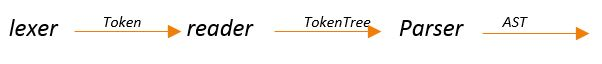
\includegraphics[width=0.8\textwidth]{images/Tokenizer.jpg}
\caption{Sweet.JS anatomy.} 
\label{fig:Tokenizer}
\end{figure}

The parser gives structure to unstructured source code. The lexer converts a character stream to a token stream and the parser converts the token stream into an abstract syntax tree (AST) according to a context free grammar ~\cite{bib2}. The macro expander  must sit between the lexer and the parser. Here the reader records sufficiently history information in the form of token trees in order to decide how to parse the token, which is required to decide if token is a divisor or a regular expression.
In traditional JavaScript compilers, the parser and lexer are intertwined; rather than running the entire program through the lexer once to get a sequence of tokens, the parser calls out to the lexer from a given grammatical context with a flag to indicate if the lexer should accept a regular expression or a divide operator and the input character are tokenized accordingly ~\cite{bib2}.
\newpage
Example

\begin{lstlisting}[frame=single]
	macro id {
  		case {_ $x } => {
   			return #{ $x }
  		}
	}
	id 42
\end{lstlisting}

\begin{figure}[htb]
\centering
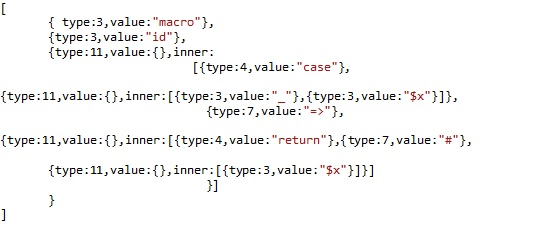
\includegraphics[width=1.0\textwidth]{images/readeroutput.jpg}
\caption{Token tree.} 
\label{fig:readeroutput}
\end{figure}
Reader convert string of token to token tree, a token tree is similar to tokens produced by the standard esprima lexer~\cite{bib7} but with the critical difference being that token trees match delimiters. 
\begin{figure}[htb]
\centering
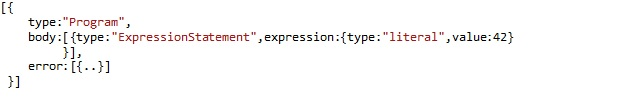
\includegraphics[width=1.0\textwidth]{images/AST.jpg}
\caption{Final AST from parser.} 
\label{fig:AST}

\end{figure}

The approach used in Sweet.JS is \textit{Enforestation}, first pioneered by Honu ~\cite{bib4}. Enforestation, extracts the sequence of terms produced by the reader to create a term tree. Consider the following \texttt{let} example 

\begin{figure}[htb]
\centering
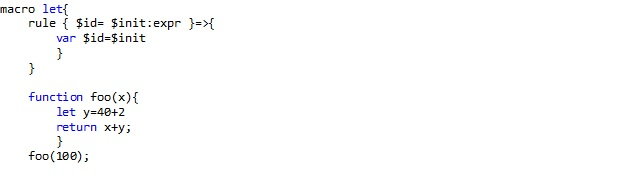
\includegraphics[width=1.0\textwidth]{images/enforest.jpg}
\caption{Macro Expansion.} 
\label{fig:AST}

\end{figure}
Enforestation begins by loading the \textit{let} as shown in Figure:4, macro into the macro environment and converting the function declaration into a term tree.

\begin{figure}[htb]
\centering
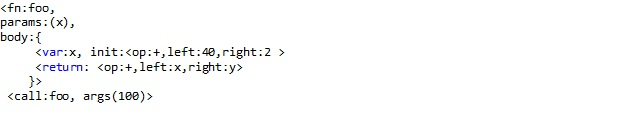
\includegraphics[width=1.0\textwidth]{images/enforest1.jpg}
\caption{Term tree.} 
\label{fig:AST}

\end{figure}

Figure 5: shows the use of \textit{let} is expanded away, \textit{var} and \textit{return} keyword is created.

A term tree is a kind of proto-AST that represent a partial parse of the program. As the expander passes through the token trees, it creates term trees that contain unexpanded sub trees that will be expanded once all macro definition have been discovered in the current scope ~\cite{bib2}.

\section{Current limitation of Sweet.JS}
\textcolor{white}{``}
Although the benefits of hygienic macros are well established, there are occasions when traditional hygienic bindings are insufficient. The classic example is "anaphoric conditionals" where the value of the tested expression is available as an \textit{it} bindings.When the condition is true, an \textit{it} identifier is automatically created and set to the value of the condition. An anaphoric macro is a type of programming macro that deliberately captures some form supplied to the macro which may be referred to by an anaphor (an expression referring to another).
\textcolor{white}{''}

\begin{figure}
\centering
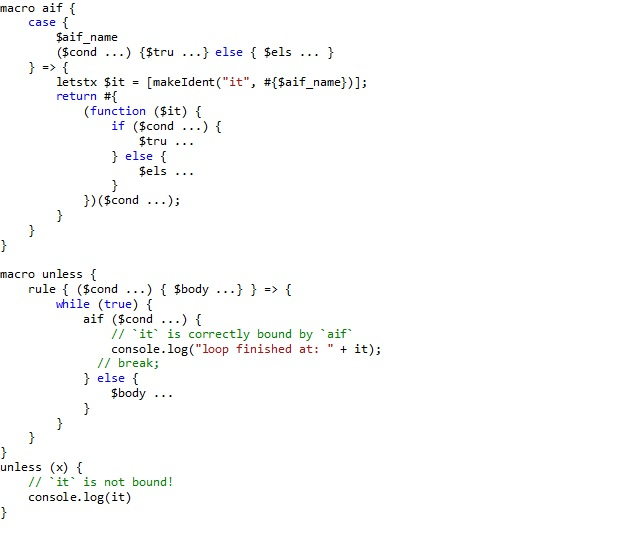
\includegraphics[width=1.0\textwidth,height=11cm]{images/Breakhygiene.jpg}
\caption{Breaking hygiene.} 
\label{fig:Breakhygiene}

\end{figure}
\newpage
In Figure 6, I define the \textit{"unless"} macro which executes code if conditional is false. If the conditional is true, code specified in the else clause is executed. Here we used \textit{anaphoric-if} condition which introduces an anaphor \textit{it} which should bind to the result of the test clause.

\begin{figure}

\centering
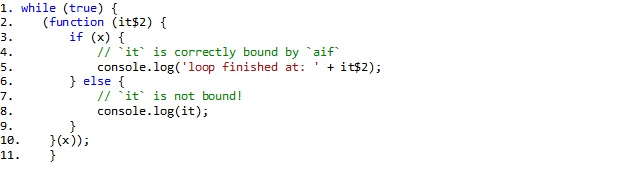
\includegraphics[width=1.0\textwidth]{images/macroexpansion.jpg}
\caption{Macro expansion.} 
\label{fig:macroexpansion}

\end{figure}

In Figure 7, on macro expansion in line (8) the identifier \texttt{it} is not defined. Here we wish to introduce the identifiers deliberately breaking hygiene. 

The same unhygienic macros are possible in Scheme as shown in the below example, 
\begin{lstlisting}[frame=single]
(define-syntax-rule (aif condition true-expr false-expr)
 (let ([it condition])
   (if it
      true-expr
      false-expr)))
aif #t (displayln it) (void))
it: undefined; //error
cannot reference an identifier before its definition
in module: 'program
\end{lstlisting}
\textcolor{white}{``}
When using syntax-parameterize, \texttt{it} acts as an alias for \texttt{tmp}. The alias behavior is created by \textbf{make-rename-transformer}. \textbf{define-syntax-parameter}, binds the keyword to the value obtained by evaluating the transformer. The transformer provides the default expansion for the syntax parameter. Usually, you will just want to have the transformer throw a syntax error indicating that the keyword is supposed to be used in conjunction with another macro as shown in the below example. 
\textcolor{white}{''}
\begin{lstlisting}[frame=single][frame=single]
(require racket/stxparam)
(define-syntax-parameter it
   (lambda (stx)
   (raise-syntax-error (syntax-e stx)
     "can only be used inside aif")))

(define-syntax-rule (aif condition true-expr false-expr)
   (let ([tmp condition])
   (if tmp
   (syntax-parameterize ([it (make-rename-transformer #'tmp)])
     true-expr)
     false-expr)))
\end{lstlisting}
\textcolor{white}{``}
\texttt{"syntax-parameterize,"} adjust keyword to use the values obtained by evaluating their transformer in the expansion of the expression. Each keyword must be bound to a syntax-parameter.
\textcolor{white}{''}
\begin{lstlisting}[frame=single][frame=single]
(aif 10 (displayln it) (void))
\end{lstlisting}
Inside the syntax-parameterize, \textit{it} acts as an alias for \textit{tmp} results of above code is 10. The alias behavior is created by \texttt{make-rename-transformer}.